\subsubsection{\NonOptimizing MSVC}

\RU{Вот что выдал MSVC 2010}\EN{MSVC 2010 generates the following}:

\lstinputlisting[caption=\NonOptimizing MSVC 2010]{patterns/12_FPU/3_comparison/x86/MSVC/MSVC.asm.\LANG}

\index{x86!\Instructions!FLD}
\RU{Итак, \FLD загружает \TT{\_b} в регистр \ST{0}.}
\EN{So, \FLD loads \TT{\_b} into \ST{0}.}

\label{Czero_etc}
\newcommand{\Czero}{\TT{C0}\xspace}
\newcommand{\Ctwo}{\TT{C2}\xspace}
\newcommand{\Cthree}{\TT{C3}\xspace}
\newcommand{\CThreeBits}{\Cthree/\Ctwo/\Czero}

\index{x86!\Instructions!FCOMP}
\RU{\FCOMP сравнивает содержимое \ST{0} с тем что лежит в \TT{\_a} и выставляет биты \CThreeBits в 
регистре статуса FPU. Это 16-битный регистр отражающий текущее состояние FPU.}
\EN{\FCOMP compares the value in \ST{0} with what is in \TT{\_a} 
and sets \CThreeBits bits in FPU 
status word register, accordingly. 
This is a 16-bit register that reflects the current state of the FPU.}

\RU{После этого, инструкция \FCOMP также выдергивает одно значение из стека. 
Это отличает её от \FCOM, которая просто сравнивает значения, оставляя стек в таком же состоянии.}
\EN{After the bits are set, the \FCOMP instruction also pops one variable from the stack. 
This is what distinguishes it from \FCOM, which is just compares values, leaving the stack in the same state.}

\RU{К сожалению, у процессоров до Intel P6 
\footnote{Intel P6 это Pentium Pro, Pentium II, и далее} нет инструкций условного перехода,
проверяющих биты \CThreeBits. 
Возможно, так сложилось исторически (вспомните о том, что FPU когда-то был вообще отдельным чипом).\\
А у Intel P6 появились инструкции \FCOMI/\FCOMIP/\FUCOMI/\FUCOMIP ~--- делающие тоже самое, 
только напрямую модифицирующие флаги \ZF/\PF/\CF.}
\EN{Unfortunately, CPUs before Intel P6
\footnote{Intel P6 is Pentium Pro, Pentium II, etc} don't have any conditional 
jumps instructions which check the \CThreeBits bits. 
Probably, it is a matter of history (remember: FPU was separate chip in past).\\
Modern CPU starting at Intel P6 have \FCOMI/\FCOMIP/\FUCOMI/\FUCOMIP 
instructions~---which do the same, but modify the \ZF/\PF/\CF CPU flags.}

\index{x86!\Instructions!FNSTSW}
\RU{Так что \FNSTSW копирует содержимое регистра статуса в \AX. 
Биты \CThreeBits занимают позиции, 
соответственно, 14, 10, 8, в этих позициях они и остаются в регистре \AX, 
и все они расположены в старшей части регистра ~--- \AH.}
\EN{The \FNSTSW instruction copies FPU the status word register to \AX. 
Bits \CThreeBits are placed at positions 14/10/8, 
they will be at the same positions in the \AX register and all they are placed in the high part of \AX{}~---\AH{}.}

\begin{itemize}
\item
\RU{Если $b>a$ в нашем случае, то биты \CThreeBits должны быть выставлены так:}
\EN{If $b>a$ in our example, then \CThreeBits bits will be set as following:} 0, 0, 0.
\item
\RU{Если $a>b$, то биты будут выставлены:}\EN{If $a>b$, then the set bits will be:} 0, 0, 1.
\item
\RU{Если $a=b$, то биты будут выставлены так:}\EN{If $a=b$, then the set bits will be:} 1, 0, 0.
\item
\RU{Если результат не определен (в случае ошибки), то биты будут выставлены так}\EN{If the result 
is unordered (in case of error), then the set bits will be}: 1, 1, 1.
\end{itemize}
% TODO: table here?

\EN{This is how \CThreeBits bits are located in the \AX register:}
\RU{Вот как биты \CThreeBits расположены в регистре \AX:}

\begin{center}
\begin{bytefield}[endianness=big,bitwidth=0.03\linewidth]{16}
\bitheader{14,10,9,8} \\
\bitbox{1}{} & 
\bitbox{1}{\TT{C3}} & 
\bitbox{3}{} & 
\bitbox{1}{\TT{C2}} & 
\bitbox{1}{\TT{C1}} & 
\bitbox{1}{\TT{C0}} &
\bitbox{8}{}
\end{bytefield}
\end{center}


\EN{This is how \CThreeBits bits are located in the \AH register:}
\RU{Вот как биты \CThreeBits расположены в регистре \AH:}

\begin{center}
\ifdefined\ebook
\begin{bytefield}[endianness=big,bitwidth=0.06\linewidth]{8}
\else
\begin{bytefield}[endianness=big,bitwidth=0.03\linewidth]{8}
\fi
\bitheader{6,2,1,0} \\
\bitbox{1}{} & 
\bitbox{1}{\TT{C3}} & 
\bitbox{3}{} & 
\bitbox{1}{\TT{C2}} & 
\bitbox{1}{\TT{C1}} & 
\bitbox{1}{\TT{C0}}
\end{bytefield}
\end{center}


\RU{После исполнения \TT{test ah, 5}\footnote{5=1001b}, % FIXME: subscript here!
будут учтены только биты \Czero и \Ctwo (на позициях 0 и 2), остальные проигнорированы.}
\EN{After the execution of \TT{test ah, 5}\footnote{5=1001b}, 
only \Czero and \Ctwo bits (on 0 and 2 position) will be considered, all other bits will be
ignored.}

\label{parity_flag}
\index{x86!\Registers!\Flags!\RU{Флаг четности}\EN{Parity flag}}
\RU{Теперь немного о \IT{parity flag}\footnote{флаг четности}. 
Еще один замечательный рудимент эпохи.}
\EN{Now let's talk about the \IT{parity flag}, another notable historical rudiment.}

\RU{Этот флаг выставляется в $1$ если количество единиц в последнем результате ~--- четно. 
И в $0$ если ~--- нечетно.}
\EN{This flag is set to $1$ if the number of ones in the result of the last calculation is even, 
and to $0$ if it is odd.}

\RU{Заглянем в}\EN{Let's look into} Wikipedia
\footnote{\href{http://go.yurichev.com/17131}{wikipedia}}:

\begin{framed}
\begin{quotation}
One common reason to test the parity flag actually has nothing to do with parity. The FPU has four condition flags 
(C0 to C3), but they can not be tested directly, and must instead be first copied to the flags register. 
When this happens, C0 is placed in the carry flag, C2 in the parity flag and C3 in the zero flag. 
The C2 flag is set when e.g. incomparable floating point values (NaN or unsupported format) are compared 
with the FUCOM instructions.
\end{quotation}
\end{framed}

\EN{As noted in Wikipedia, the parity flag used sometimes in FPU code, let's see how.}
\RU{Как упоминается в Wikipedia, флаг четности иногда используется в FPU-коде и сейчас увидим, как.}

\index{x86!\Instructions!JP}
\RU{Флаг \PF будет выставлен в $1$, если \Czero и \Ctwo 
оба $1$ или оба $0$. 
И тогда сработает последующий \JP (\IT{jump if PF==1}). 
Если мы вернемся чуть назад и посмотрим значения \CThreeBits 
для разных вариантов, то увидим, что условный переход \JP сработает в двух случаях: если $b>a$ или если $a=b$ 
(ведь бит \Cthree перестал учитываться после исполнения \TT{test ah, 5}).}
\EN{The \PF flag will be set to 1 if both \Czero and \Ctwo are set to $0$ or both are $1$, in which case
the subsequent \JP (\IT{jump if PF==1}) will trigger. 
If we recall the values of \CThreeBits for various cases,
we can see that the conditional jump 
\JP will be triggered in two cases: if $b>a$ or $a=b$ 
(\Cthree bit is not considered here, since it was cleared by 
the \TT{test ah, 5} instruction).}

\RU{Дальше все просто. Если условный переход сработал, то \FLD загрузит значение \TT{\_b} в \ST{0}, 
а если не сработал, то загрузится \TT{\_a} и произойдет выход из функции.}
\EN{It is all simple after that. If the conditional jump was triggered, \FLD will load the value of \TT{\_b} 
in \ST{0}, and if it was not triggered, the value of \TT{\_a} will be loaded there.}

\myparagraph{\RU{А как же проверка флага \Ctwo}\EN{And what about checking \Ctwo}?}

\RU{Флаг \Ctwo включается в случае ошибки (\gls{NaN}, и т.д.), но наш код его не проверяет.}
\EN{The \Ctwo flag is set in case of error (\gls{NaN}, etc), but our code doesn't check it.}
\RU{Если программисту нужно знать, не произошла ли FPU-ошибка, он должен позаботиться об этом
дополнительно, добавив соответствующие проверки.}
\EN{If the programmer cares about FPU errors, he/she must add additional checks.}

\ifdefined\IncludeOlly
\clearpage
\myparagraph{\RU{Первый пример с \olly}\EN{First \olly example}: a=1.2 \AndENRU b=3.4}
\index{\olly}

\RU{Загружаем пример в}\EN{Let's load the example into} \olly:

\begin{figure}[H]
\centering
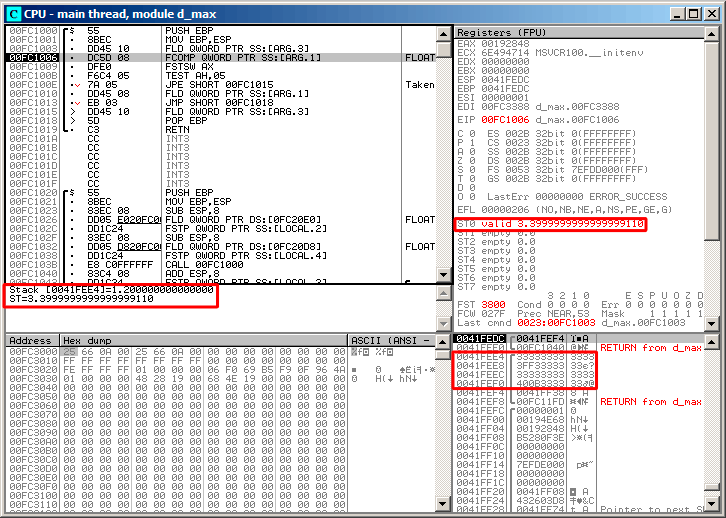
\includegraphics[scale=\FigScale]{patterns/12_FPU/3_comparison/x86/MSVC/olly1_1.png}
\caption{\olly: \RU{первая \FLD исполнилась}\EN{first \FLD is executed}}
\label{fig:FPU_comparison_case1_olly1}
\end{figure}

\RU{Текущие параметры ф-ции}\EN{Current arguments of the function}: $a=1.2$ \AndENRU $b=3.4$ 
(\RU{их видно в стеке: 2 пары 32-битных значений}\EN{We can see them in the stack: two pairs of 32-bit values}).
$b$ ($3.4$) \RU{уже загружено в}\EN{is already loaded in} \ST{0}.
\RU{Сейчас будет исполняться \FCOMP}\EN{Now \FCOMP will be executed}. 
\olly \RU{показывает второй аргумент для \FCOMP, который сейчас находится в стеке}\EN{shows the second \FCOMP
argument, which is in stack right now}.

\clearpage
\FCOMP \RU{отработал}\EN{is executed}:

\begin{figure}[H]
\centering
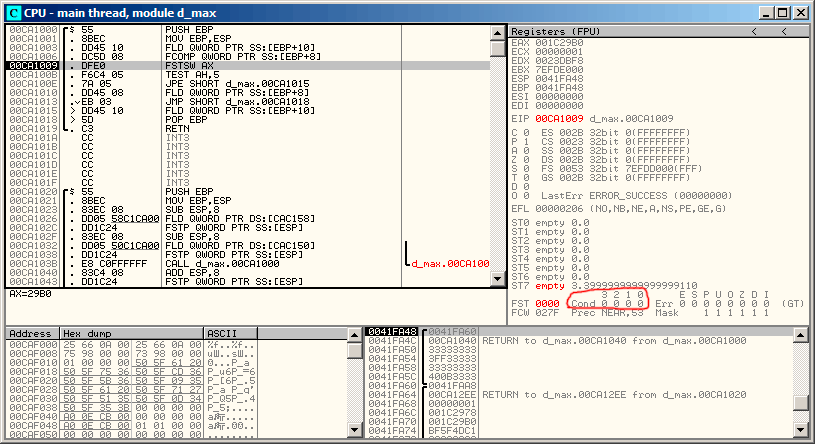
\includegraphics[scale=\FigScale]{patterns/12_FPU/3_comparison/x86/MSVC/olly1_2.png}
\caption{\olly: \FCOMP \RU{исполнилась}\EN{is executed}}
\label{fig:FPU_comparison_case1_olly2}
\end{figure}

\RU{Мы видим состояния condition-флагов \ac{FPU}}\EN{We see the state of the \ac{FPU}'s condition flags}: 
\RU{все нули}\EN{all zeroes}.
\RU{Вытолкнутое значение отображается как \ST{7}, почему это так, я писал раннее}
\EN{The popped value is reflected as \ST{7}, I wrote earlier about reason for this}: 
\ref{FPU_is_rather_circular_buffer}.

\clearpage
\FNSTSW \RU{сработал}\EN{is executed}:
\begin{figure}[H]
\centering
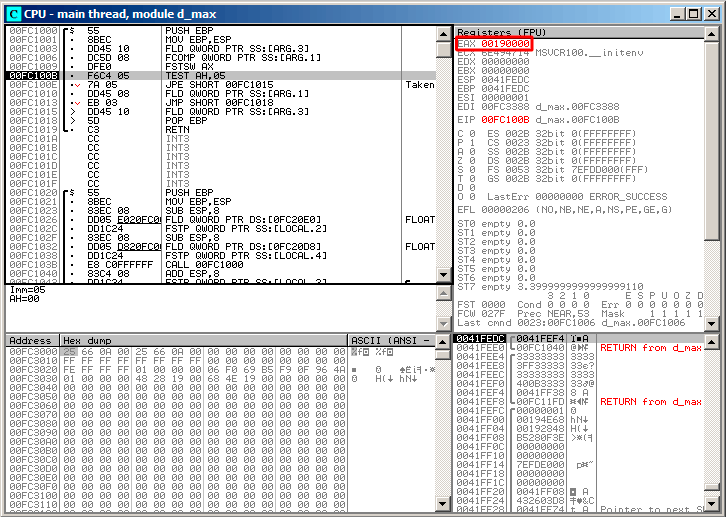
\includegraphics[scale=\FigScale]{patterns/12_FPU/3_comparison/x86/MSVC/olly1_3.png}
\caption{\olly: \FNSTSW \RU{исполнилась}\EN{is executed}}
\label{fig:FPU_comparison_case1_olly3}
\end{figure}

\RU{Видно, что регистр \TT{AX} содержит нули: действительно, ведь все condition-флаги тоже содержали нули.}
\EN{We see that the \TT{AX} register contain zeroes: indeed, all condition flags are zero.}
(\olly \RU{дизассемблирует команду}\EN{disassembles the} \FNSTSW \RU{как}\EN{instruction as} \TT{FSTSW} --- 
\RU{это синоним}\EN{they are synonyms}).

\clearpage
\TEST \RU{сработал}\EN{is executed}:

\begin{figure}[H]
\centering
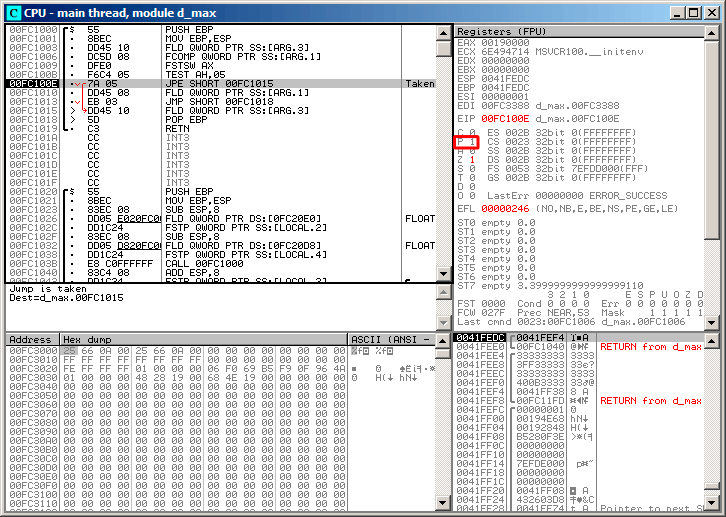
\includegraphics[scale=\FigScale]{patterns/12_FPU/3_comparison/x86/MSVC/olly1_4.png}
\caption{\olly: \TEST \RU{исполнилась}\EN{is executed}}
\label{fig:FPU_comparison_case1_olly4}
\end{figure}

\RU{Флаг \TT{PF} равен единице.}\EN{The \TT{PF} flag is set to $1$.}
\RU{Все верно: количество выставленных бит в $0$ --- это $0$, а $0$ --- это четное число.}
\EN{Indeed: the number of bits set in $0$ is $0$ and $0$ is an even number.}
\olly \RU{дизассемблирует}\EN{disassembles} \TT{JP} \RU{как}\EN{as} \ac{JPE} --- \RU{это синонимы}\EN{they
are synonyms}.
\RU{И она сейчас сработает}\EN{And it will trigger now}.

\clearpage
\ac{JPE} \RU{сработала}\EN{triggered}, \FLD \RU{загрузила в \ST{0} значение $b$ ($3.4$)}
\EN{loads the value of $b$ ($3.4$) in \ST{0}}:

\begin{figure}[H]
\centering
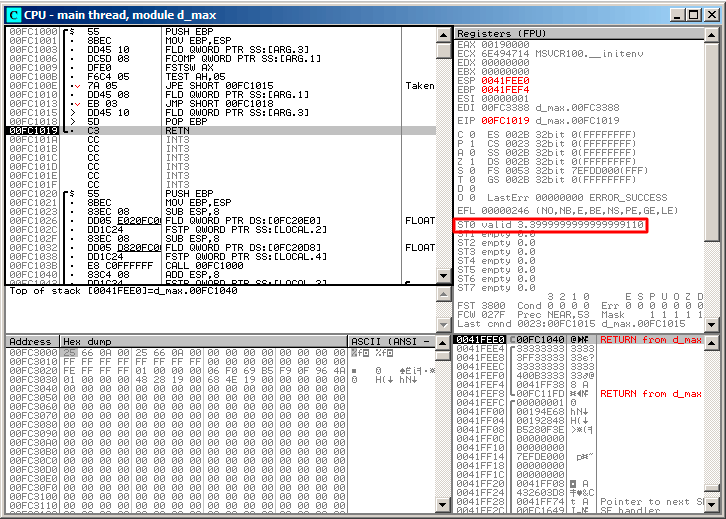
\includegraphics[scale=\FigScale]{patterns/12_FPU/3_comparison/x86/MSVC/olly1_5.png}
\caption{\olly: \RU{вторая \FLD исполнилась}\EN{second \FLD is executed}}
\label{fig:FPU_comparison_case1_olly5}
\end{figure}

\RU{Ф-ция заканчивает свою работу}\EN{The function finishes its work}.

\clearpage
\myparagraph{\RU{Второй пример с \olly}\EN{Second \olly example}: a=5.6 \AndENRU b=-4}

\RU{Загружаем пример в}\EN{Let's load example into} \olly:

\begin{figure}[H]
\centering
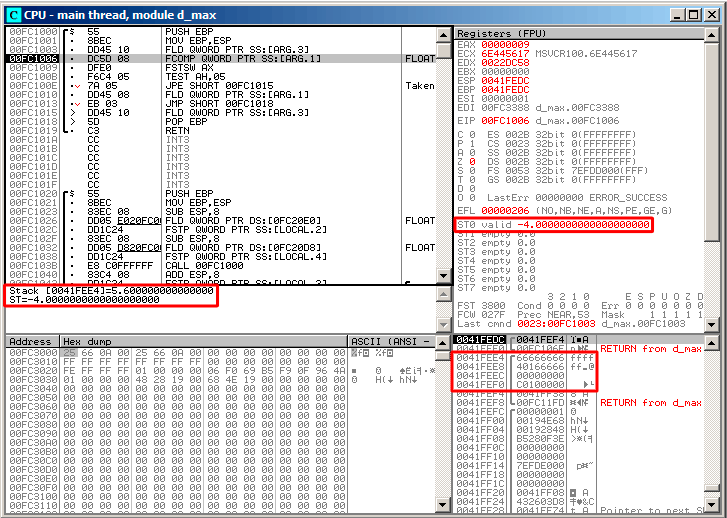
\includegraphics[scale=\FigScale]{patterns/12_FPU/3_comparison/x86/MSVC/olly2_1.png}
\caption{\olly: \RU{первая \FLD исполнилась}\EN{first \FLD executed}}
\label{fig:FPU_comparison_case2_olly1}
\end{figure}

\RU{Текущие параметры ф-ции}\EN{Current function arguments}: $a=5.6$ \AndENRU $b=-4$).
$b$ ($-4$) \RU{уже загружено в}\EN{is already loaded in} \ST{0}.
\RU{Сейчас будет исполняться \FCOMP}\EN{\FCOMP will execute now}. 
\olly \RU{показывает второй аргумент \FCOMP, который сейчас находится в стеке}
\EN{shows the second \FCOMP argument, which is in stack right now}.

\clearpage
\FCOMP \RU{отработал}\EN{executed}:

\begin{figure}[H]
\centering
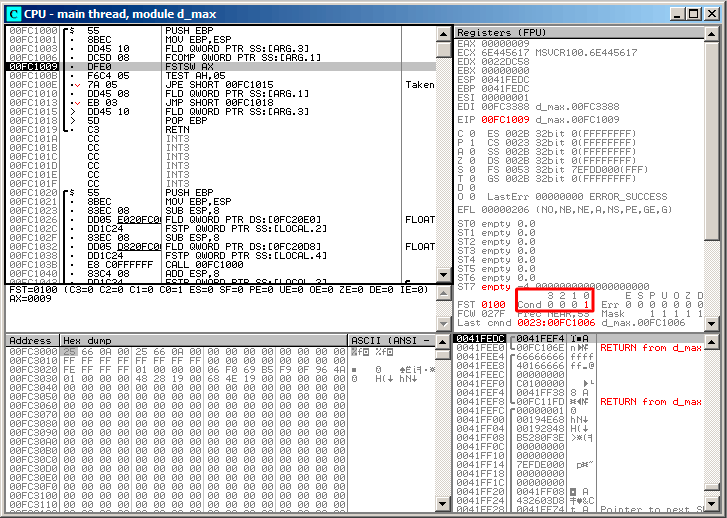
\includegraphics[scale=\FigScale]{patterns/12_FPU/3_comparison/x86/MSVC/olly2_2.png}
\caption{\olly: \FCOMP \RU{исполнилась}\EN{executed}}
\label{fig:FPU_comparison_case2_olly2}
\end{figure}

\RU{Мы видим значения condition-флагов \ac{FPU}: все нули кроме \Czero.}
\EN{We see the state of the \ac{FPU}'s condition flags: all zeroes except \Czero.}

\clearpage
\FNSTSW \RU{сработал}\EN{executed}:

\begin{figure}[H]
\centering
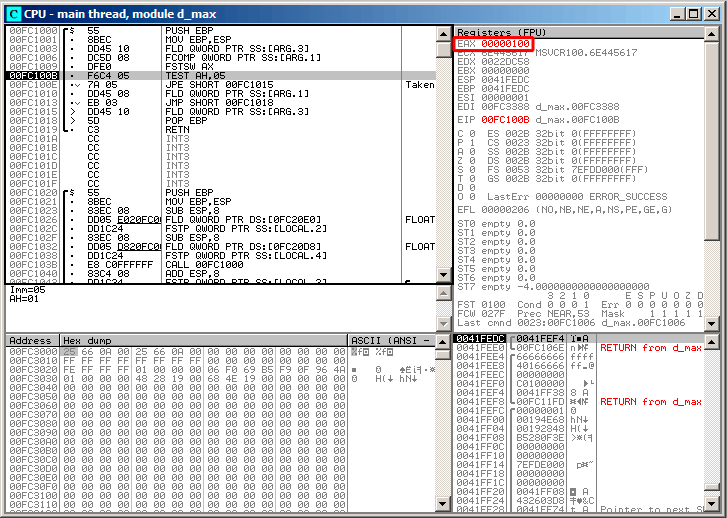
\includegraphics[scale=\FigScale]{patterns/12_FPU/3_comparison/x86/MSVC/olly2_3.png}
\caption{\olly: \FNSTSW \RU{исполнилась}\EN{executed}}
\label{fig:FPU_comparison_case2_olly3}
\end{figure}

\RU{Видно, что регистр \TT{AX} содержит \TT{0x100}: флаг \Czero стал на место 16-го бита.}
\EN{We see that the \TT{AX} register contains \TT{0x100}: the \Czero flag is at the 16th bit.}

\clearpage
\TEST \RU{сработал}\EN{executed}:

\begin{figure}[H]
\centering
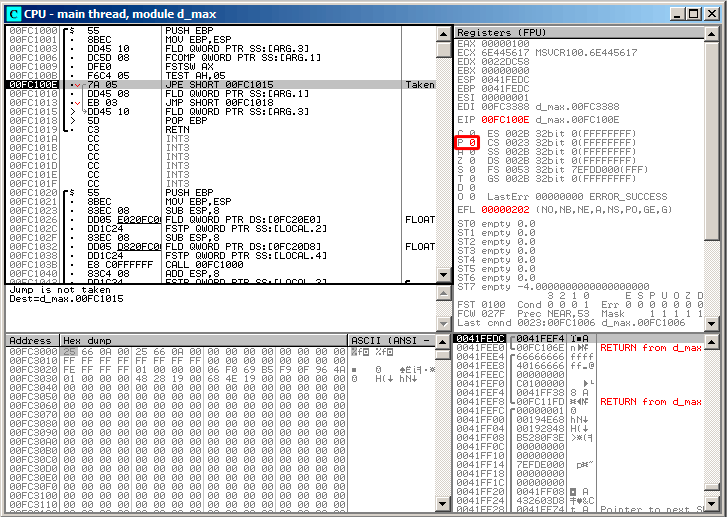
\includegraphics[scale=\FigScale]{patterns/12_FPU/3_comparison/x86/MSVC/olly2_4.png}
\caption{\olly: \TEST \RU{исполнилась}\EN{executed}}
\label{fig:FPU_comparison_case2_olly4}
\end{figure}

\EN{The}\RU{Флаг} \TT{PF} \RU{равен нулю}\EN{ flag is cleared}.
\RU{Все верно}\EN{Indeed}: 
\RU{количество единичных бит в \TT{0x100} --- это $1$, а $1$ --- это нечетное число}
\EN{the count of bits set in \TT{0x100} is $1$ and $1$ is an odd number}.
\ac{JPE} \RU{сейчас не сработает}\EN{will not be triggered}.

\clearpage
\ac{JPE} \RU{не сработала, }\EN{wasn't triggered, so} \FLD 
\RU{загрузила в \ST{0} значение $a$ ($5.6$)}
\EN{loads the value of $a$ ($5.6$) in \ST{0}}:

\begin{figure}[H]
\centering
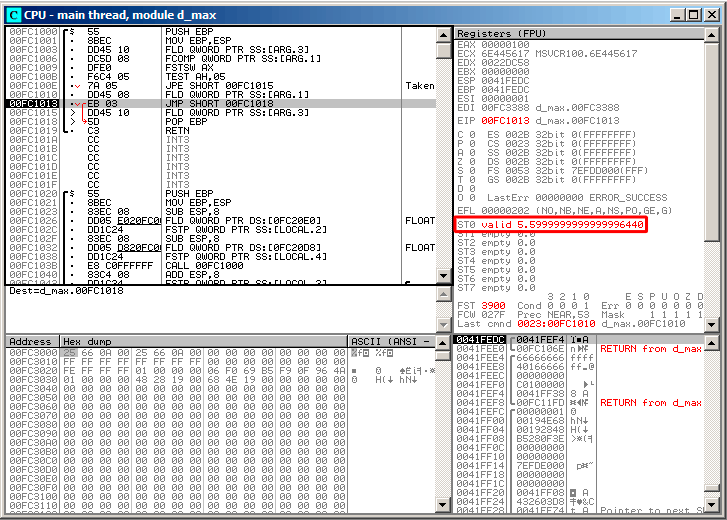
\includegraphics[scale=\FigScale]{patterns/12_FPU/3_comparison/x86/MSVC/olly2_5.png}
\caption{\olly: \RU{вторая \FLD исполнилась}\EN{second \FLD executed}}
\label{fig:FPU_comparison_case2_olly5}
\end{figure}

\RU{Ф-ция заканчивает свою работу}\EN{The function finishes its work}.

\fi
